\chapter{Обзор литературы}

\section{Когерентный контроль}

\begin{figure}[b!]
    \begin{center}
        \includegraphics[width=\textwidth]{pictures/Coherent_Control.png}
        \caption{Принципиальная схема эксперимента, реализующего когерентный контроль. Два когерентных встречных пучка A и B падают на структуру субволновой толщины, например, на пленку плазмонного метаматериала. Существуют два случая, при которых пучки на пленке интерферируют либо деструктивно \textbf{(А)}, либо конструктивно \textbf{(Б)}, вызывая пропускание или поглощение соответственно\cite{lightWithLight2012}.}
        \label{fig:coherentControl}
    \end{center}
\end{figure}

Метод когерентного контроля в общем случае заключается в изучении интерференционной картины, полученной после взаимодействия двух когерентных пучков, распространяющихся в противоположных направлениях, с оптически неоднородной средой (Рис. \ref{fig:coherentControl}). При таком взаимодействии в пространстве образуется стоячая электромагнитная волна, и степень влияния неоднородности на интерференционную картину определяется положением пучностей и узлов относительно структуры, которое можно контролировать с помощью изменения фаз одного из источников. При рассмотрении сред, линейные размеры которых по направлению распространения излучения (толщина) значительно меньше длины волны, можно выделить два предельных случая\cite{lightWithLight2015}:
\begin{enumerate}
    \item Когерентное полное пропускание (CPT, англ. <<coherent perfect transmission>>). Структура находится в узле стоячей волны. Тогда неоднородность становится <<выключенной>> и практически не влияет на распространение излучения.
    \item Когерентное полное поглощение (CPA, англ. <<coherent perfect absorption>>). Структура находится в пучности. Тогда влияние неоднородности максимально.
\end{enumerate}
За счёт этих двух состояний можно реализовывать полностью оптическое переключение, а также базовые логические операции: сложение, вычитание и умножение (Рис. \ref{fig:opticalLogic}). Также когерентный контроль позволяет модулировать интенсивность в широких пределах\cite{lightWithLight2012}, создавать оптические транзисторы\cite{lightWithLight2015}, измерять поглощение и другие характеристики материалов неразрушающим путем\cite{CPAGraphene2017} и многое другое.

\begin{figure}
    \begin{center}
        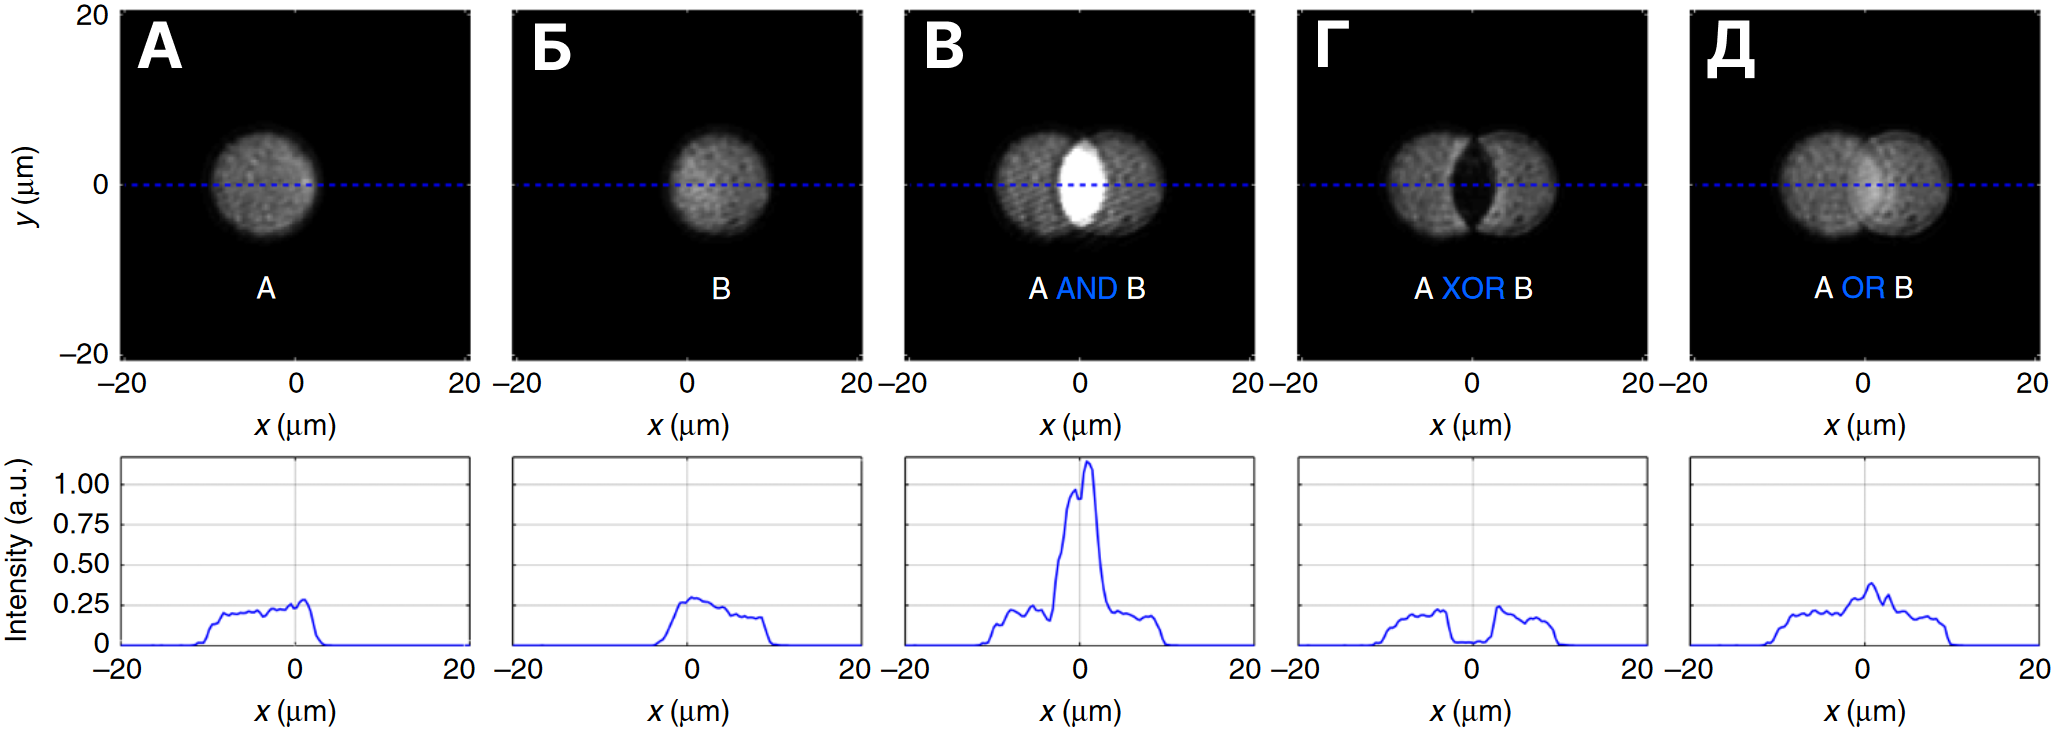
\includegraphics[width=\textwidth]{pictures/Optical_logic.png}
        \caption{Оптические базовые логические операции. Изображения метаповерхности, \textbf{(А)} освещенной только лучом $A$, \textbf{(Б)} только лучом $B$ и \textbf{(В-Д)} обоими лучами $A$ и $B$. Разным относительным фазам лучей $A$ и $B$ соответствуют разные логические операции: \textbf{(В)} $A$ И $B$ ($\Theta = \pi$), \textbf{(Г)} $A$ <<ИСКЛЮЧАЮЩЕЕ ИЛИ>> $B$ ($\Theta = 0$) и \textbf{(Д)} $A$ ИЛИ $B$ ($\Theta = \pm \pi/3$). На нижних графиках показан профиль интенсивности вдоль соответствующей пунктирной синей линии. Уровни интенсивности показаны в одинаковых оттенках серого на всех изображениях и в одном вертикальном масштабе на всех графиках\cite{twoDimensional2016}.}
        \label{fig:opticalLogic}
    \end{center}
\end{figure}

Теоретически метод когерентного контроля можно описать с помощью комплексной матрицы рассеяния. Пусть два когерентных оптических пучка $E_\alpha$ и $E_\beta$, распространяющихся в противоположных направлениях, падают по нормали на некоторый слой материала с линейными оптическими характеристиками и пусть при взаимодействии с материалом сохраняется поляризация излучения. Две результирующие волны (по обе стороны от плоскости материала) обозначим $E_\delta$ и $E_\gamma$. Тогда соответствующие напряженности электрических полей связаны матрицей рассеяния $\mathbf{S}$:
\begin{equation}
    \begin{bmatrix}
        E_\delta \\
        E_\gamma
    \end{bmatrix} = \begin{bmatrix}
        S_{11} & S_{12} \\
        S_{21} & S_{22}
    \end{bmatrix} \begin{bmatrix}
        E_\alpha \\
        E_\beta
    \end{bmatrix}.
    \label{eq:scatteringMatrix}
\end{equation}
Аналитические выражения для коэффициентов $S_{ij}$, которые зависят от характеристик материала, приводятся в \cite{CPATheory2015}.

\begin{figure}
    \begin{center}
        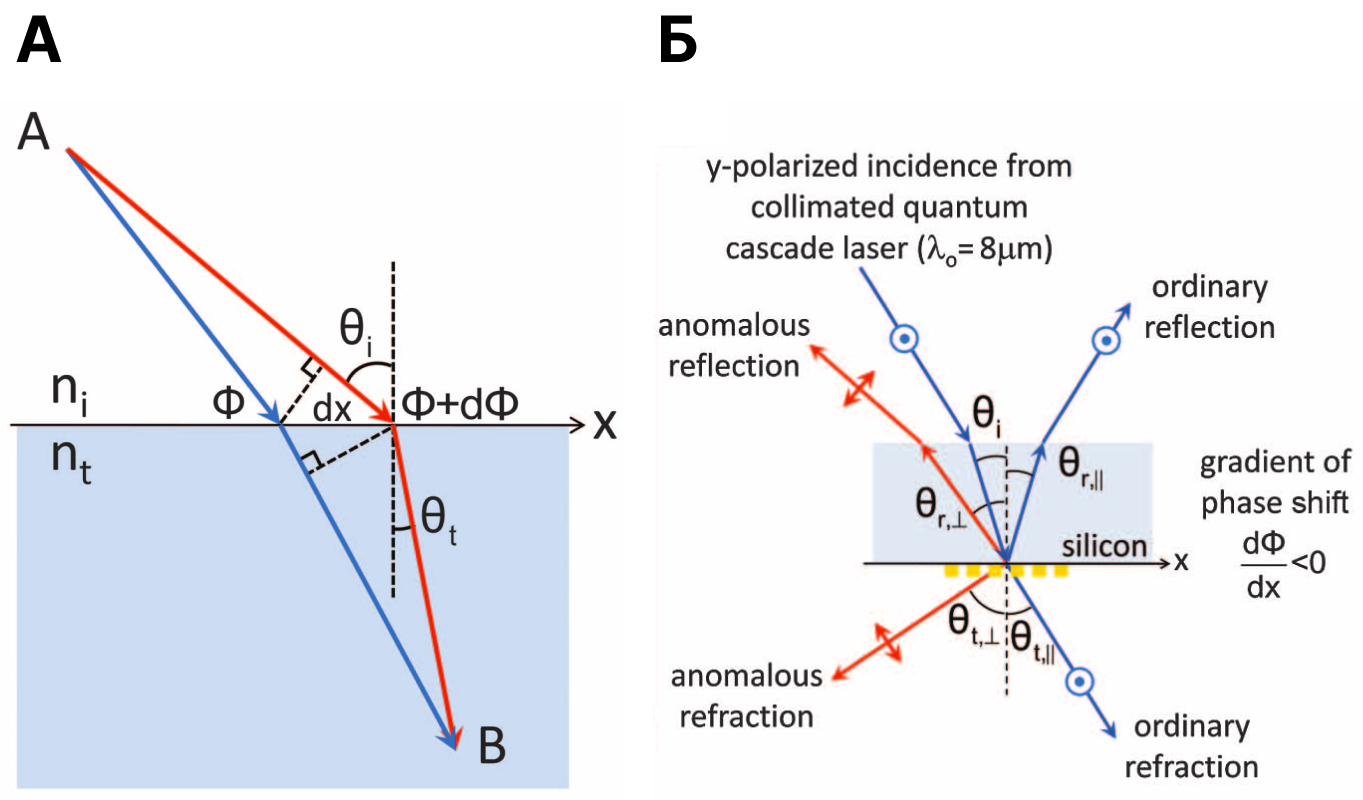
\includegraphics[width=\textwidth]{pictures/Generalized_Snell's_law.png}
        \caption{\textbf{(А)} Рисунок, используемый для вывода обобщенного закона преломления Снеллиуса. Граница между двумя средами искусственно структурирована так, чтобы внести резкий фазовый градиент на пути света, который зависит от положения на границе раздела. $\Phi$ и $\Phi + d\Phi$ — фазовые сдвиги, при которых два луча (синий и красный) пересекают границу\cite{generalized2011}. \textbf{(Б)} Схема эксперимента, демонстрирующего обобщенный закон Снеллиуса\cite{generalized2011}.}
        \label{fig:generalized}
    \end{center}
\end{figure}

\section{Обобщенный закон Снеллиуса}
В качестве оптически неоднородных сред могут быть использованы структуры, у которых фаза меняется вдоль границы раздела, как показано на Рис. \ref{fig:generalized}А. Приведем теоретические основы физики таких структур.

Пусть каждой точке $M(x)$ границы раздела вдоль оси $\mathrm{X}$ соответствует значение фазы, равное $\Phi(x)$ и пусть падающая на границу раздела волна, проходящая через заданную точку $M(x)$, претерпевает фазовый разрыв $d\Phi(x)$. Для такой границы мы вынуждены пересмотреть классический закон Снеллиуса, описываемый формулой:
\begin{equation}
    n_i \sin \Theta_i = n_t \sin \Theta_t,
\end{equation}
в соответствии с принципом Ферма.

Рассмотрим плоскую волну, падающую под углом $\Theta_i$ . Если предположить, что два пути бесконечно близки к реальному пути света (Рис. \ref{fig:generalized}А), то разность фаз между ними равна нулю:
\begin{equation}
    \label{eq:opticalPathLengthDifference}
    [k_0n_i\sin\Theta_i\, dx + (\Phi + d\Phi)] - [k_0n_t\sin\Theta_t\,dx + \Phi] = 0,
\end{equation}
где $\Theta_t$ --- угол преломления; $\Phi$ и $\Phi + d\Phi$ --- разрывы фаз в местах пересечения границы раздела синим и красным путями соответственно; $dx$ --- расстояние между точками пересечения; $n_i$ и $n_t$ --- показатели преломления двух сред; $k_0 = 2\pi/\lambda_0$ --- волновое число, где $\lambda_0$ --- длина волны в вакууме. Если градиент фазы $d\Phi/dx$ создан постоянным, предыдущее уравнение \eqref{eq:opticalPathLengthDifference} приводит к обобщенному закону преломления Снеллиуса\cite{generalized2011}:
\begin{equation}
    \label{eq:generalizedRefraction}
    n_t\sin\Theta_t - n_i \sin\Theta_i = \frac{\lambda_0}{2\pi}\frac{d\Phi}{dx}.
\end{equation}

Выражение \eqref{eq:generalizedRefraction} показывает, что преломленный луч может иметь произвольное направление при условии, что создан подходящий постоянный градиент фазы $d\Phi/dx$ вдоль границы раздела (Рис.~\ref{fig:generalized}Б). Более того, при ненулевом градиенте фазы два угла падения $\pm \Theta_i$ соответствуют различным углам преломления. Как следствие, существуют два угла полного внутреннего отражения:
\begin{equation}
    \Theta_c = \arcsin \left(\pm\frac{n_t}{n_i} - \frac{\lambda_0}{2\pi}\frac{d\Phi}{dx}\right).
\end{equation}
Аналогично, для отражения имеем:
\begin{equation}
    \label{eq:generalizedReflection}
    \sin\Theta_r - \sin\Theta_i = \frac{\lambda_0}{2\pi n_i}\frac{d\Phi}{dx},
\end{equation}
где $\Theta_r$ --- угол отражения. Между $\Theta_r$ и $\Theta_i$ существует нелинейная связь, которая заметно отличается от известного закона геометрической оптики. Уравнение \eqref{eq:generalizedReflection} показывает, что всегда существует критический угол падения:
\begin{equation}
    \Theta_c' = \arcsin\left(1 - \frac{\lambda_0}{2\pi n_i}\left|\frac{d\Phi}{dx}\right|\right),
\end{equation}
при котором отраженная волна становится эванесцентной.

В настоящее время для создания градиента по фазе используются метаповерхности, представляющие собой двумерные массивы оптических резонансных элементов --- антенн (Рис. \ref{fig:generalized}Б). Тонкая настройка размеров и формы антенн позволяет задавать фазовый градиент и тем самым изменять направление распространения пучка. Таким образом обобщенный закон Снеллиуса открывает широкие возможности для управления распространением света.


\section{Управление распространением света}

Способность направлять оптические лучи имеет решающее значение для современных технологий. Среди них — лидар (англ. LiDAR, Light Detection and Ranging, «обнаружение и определение дальности с помощью света»)\cite{jaboyedoff2012use}, лазерная визуализация\cite{holmstrom2014mems}, атмосферная оптическая линия связи (АОЛС)\cite{khalighi2014survey} и однопиксельная визуализация\cite{edgar2019principles}. Ранние методы предполагали механическое и электрическое управление оптическими элементами: повороты и перемещения зеркал и линз, изменение показателя преломления жидкого кристалла под действием приложенного напряжения и т. д.\cite{tholl2006novel}. Однако такие устройства были громоздкими и ограниченными в скорости и надежности. Развитие технологий изготовления структур нанометровых масштабов и успехи в исследовании взаимодействия света с ними позволяют создавать более эффективные и производительные полностью оптические системы.

\subsection{Характеристики способов управления.}
Для достижения параметров, необходимых для реальных приложений, системы управления должны обладать определенными характеристиками. А именно, пучок должен быть достаточно узким, иметь высокое угловое разрешение и подчиняться управлению в большом диапазоне углов, называемом полем зрения (FOV, field of view): вплоть до 180° для одномерного сканирования и до полусферы для двумерного сканирования. Кроме того, угол излучения должен перенастраиваться в реальном времени на высокой скорости с минимальными потерями интенсивности. В настоящее время существует несколько способов управления пучком, основанных на методе когерентного контроля: активные метаповерхности, медленное световое сканирование и оптические фазовые антенные решетки (ФАР). Рассмотрим эти способы подробнее.

\begin{figure}
    \begin{center}
        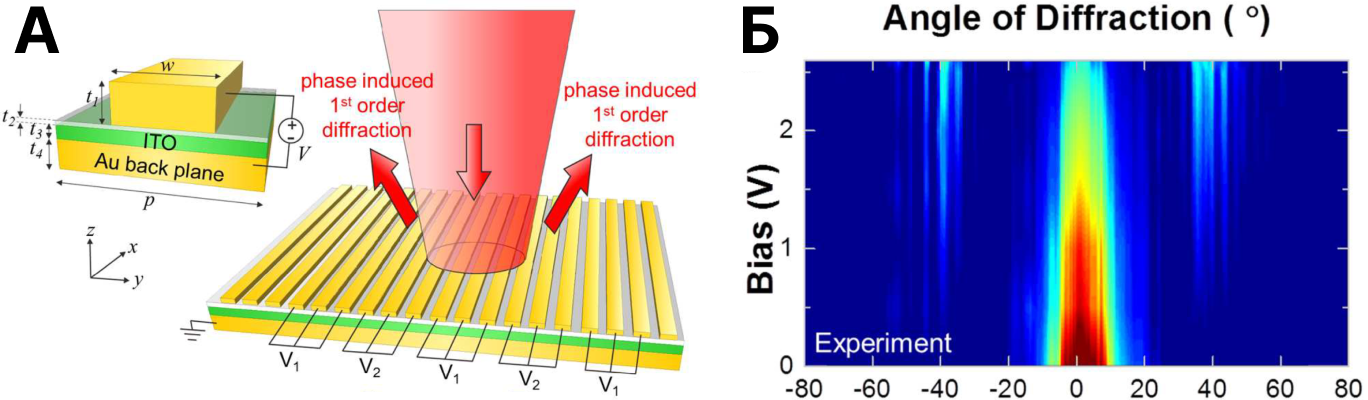
\includegraphics[width=\textwidth]{pictures/Metasurfaces.png}
        \caption{\textbf{(А)} Схема активной метаповерхности. Структура состоит из
            кварцевой подложки, золотой пластины-основания, тонкой пленки ITO (англ. <<indium tin oxide>>, оксид индия-олова), за которой следует тонкая пленка Al\textsubscript{2}O\textsubscript{3}, на которой создана периодическая структура наноантенн из золотых полосок. Напряжение подается между полосчатой антенной и золотым слоем, что приводит к накоплению заряда на границе раздела Al\textsubscript{2}O\textsubscript{3}/ITO\cite{huang2016gate}. \textbf{(Б)} Экспериментально измеренный профиль интенсивности дальнего поля для данной метаповерхности\cite{huang2016gate}.}
        \label{fig:metasurfaces}
    \end{center}

\end{figure}

\subsection{Метаповерхности.}
Как было сказано в параграфе 2, метаповерхности представляют собой структуры субволновых оптических элементов --- антенн, реализующих фазовый градиент для падающей плоской волны, определяемый геометрией антенн и характеристиками материала изготовления метаповерхности. В соответствии с обобщенным законом Снеллиуса, за счёт наличия градиента фазы наблюдается как нормальный прошедший пучок, так и аномальный (Рис. \ref{fig:metasurfaces}А), отклоняющийся на угол, определяемый выражением \eqref{eq:generalizedReflection}. Так, в работе\cite{huang2016gate} с помощью активной метаповерхности экспериментально осуществлялась <<перекачка>> интенсивности между нулевым и $\pm1$ порядками дифракции, распространяющимися под углом 40° к нормали (Рис. \ref{fig:metasurfaces}Б).

\begin{figure}
    \begin{center}
        \includegraphics[width=\textwidth]{pictures/Slow_Light.png}
        \caption{\textbf{(А)} Схематичное изображение предложенного устройства управления световым пучком с помощью медленного света с VCSEL-резонатором. Свет падает на торец и усиливается вдоль резонатора\cite{gu2011giant}. \textbf{(Б)} ФАР с использованием титановых нагревателей с линейно возрастающей длиной волноводов по всей решетке, изготовленная на КНИ (<<кремний на изоляторе>>)\cite{van2009off}.}
        \label{fig:slowLight}
    \end{center}
\end{figure}

\subsection{Пространственное сканирование на основе эффекта медленного света.}
Физические принципы устройств управления с помощью эффекта медленного света проиллюстрированы в работе\cite{gu2011giant}. Медленный свет --- это излучение, фазовая скорость которого сильно меньше, чем в вакууме. Такие состояния обычно реализуются в фотонно-кристаллических волноводах и имеют сильную дисперсию, что используется для контроля направления распространения оптического пучка.

Изначально задуманная архитектура устройства напоминает вертикально излучающий лазер (VCSEL, англ. <<vertical-cavity surface emitting laser>>) (Рис. \ref{fig:slowLight}А). Один конец конструкции открыт для прохождения света в брэгговское зеркало. Результирующая волноводная мода ограничена полным внутренним отражением сбоку, а сверху и снизу --- брэгговским отражением. Верхнее брэгговское зеркало частично пропускает излучение. Расчеты авторов показали, что благодаря сильной дисперсии моды угол излучения можно регулировать более чем на 70°, изменяя длину волны входного сигнала в диапазоне от 940 до 980 нм.


\subsection{Оптические фазовые антенные решетки.}
Общий принцип работы устройств, использующих ФАР, заключается в следующем. Свет подается в первичный волновод, и несколько светоделителей поровну перераспределяют энергию по многим вторичным оптическим каналам. В каждом из каналов осуществляется контроль фазы с помощью элементов, наносимых на волноводы. Это могут быть электрооптические и термические материалы, которые позволяют менять показатель преломления под действием внешних воздействий (например, электрического тока). Можно спроектировать архитектуру устройства таким образом, чтобы она создавала фазовый градиент по всей сетке волноводов, а сдвинутые по фазе моды волновода интерферировали во внешнюю среду через выводные дифракционные решетки (Рис. \ref{fig:slowLight}Б). Лучшая разработка имеет возможность осуществлять двумерный контроль распространения пучка и обладает существенным полем зрения в 80°x17°\cite{hutchison2016high}.

\subsection{Сравнительная таблица}
В Табл. \ref{tab:comparison} приведены сравнительные характеристики устройств контроля направления распространения оптического излучения, реализованных на практике. К ключевым характеристикам относят: угол обзора (FOV), угловое разрешение, угловую расходимость пучка, скорость изменения направления и энергопотребление.

Представленные активные метаповерхности имеют сложные электрические схемы и могут осуществлять лишь дискретное переключение угла отклонения пучка, что делает их неактуальными для задач непрерывного контроля. В устройствах, основанных на эффекте медленного света необходимо непрерывно изменять длину волны для отклонения пучка, что также существенно ограничивает область их применения. ФАР используют сложные электрооптические схемы и затруднительны в изготовлении. В то же время когерентный контроль представляет простой способ для контроля взаимодействия света с оптической резонансной структурой. С помощью него была показана возможность непрерывного управления углом распространения пучка.
\begin{table}[h]
    \caption{Сравнительная таблица характеристик устройств контроля направления распространения оптического излучения. Все значения получены экспериментально, за исключением значений в круглых скобках, которые выведены косвенно. Для метаповерхностей потребление указано для всей метаповерхности на максимальной скорости, для других устройств указано потребление \textit{одной} антенны. Адаптировано из \cite{lin_high-performance_2022}.}
    \scriptsize{
        \begin{tabular}[width=\textwidth]{|l|r|r|r|r|r|r|}
            \hline
                                                                      & Ссылка                       & FOV, ° & Разрешение & Расходимость, ° & Скорость, МГц & Потребление, мВт \\
            \hline
            \multirow{4}{*}{\parbox{53pt}{Ме\-та\-по\-вер\-хно\-сти}} & \cite{huang2016gate}         & 40     & -          & (2)             & >10           & (700)            \\
                                                                      & \cite{sokhoyan2020electro}   & 44x0   & 9x1        & (2x2)           & -             & -                \\
                                                                      & \cite{wu2019dynamic}         & 12     & -          & (0,8)           & -             & -                \\
                                                                      & \cite{park2021all}           & 6      & 31         & 0,2             & 5,4           & (96)             \\
            \hline
            \multirow{4}{*}{\parbox{53pt}{Мед\-лен\-ный свет}}        & \cite{gu2011giant}           & 70     & >1000      & 0,025           & -             & -                \\
                                                                      & \cite{kondo2017fan}          & 23     & 100        & 0,23            & -             & -                \\
                                                                      & \cite{takeuchi2018thermally} & 21     & 120        & 0,2             & 0,1           & 1300             \\
                                                                      & \cite{ito2020wide}           & 40x4,4 & 266x40     & 0,15x0,15       & -             & -                \\
            \hline
            \multirow{4}{*}{\parbox{53pt}{ФАР}}                       & \cite{hulme2015fully}        & 23x3,6 & (23x6)     & 1x0,6           & 0,3           & 160              \\
                                                                      & \cite{hutchison2016high}     & 80x17  & 570x120    & 0,140x0,142     & -             & -                \\
                                                                      & \cite{fatemi2019nonuniform}  & 16x16  & (20x20)    & 0,8x0,8         & 0,019         & 10,6             \\
                                                                      & \cite{poulton2019long}       & 56x15  & (1400x375) & 0,04x0,04       & 0,033         & 0,002            \\
                                                                      & \cite{dostart2020serpentine} & 70x6   & (470x75)   & 0,15x0,08       & 0,15          & 1,7              \\
            \hline
        \end{tabular}}
    \label{tab:comparison}
\end{table}



